\documentclass[aspectratio=1610,onlymath]{beamer}
% \documentclass[aspectratio=1610,onlymath,handout]{beamer}

\input{macros-lecture}
% Common notation

\usepackage{amsmath,amssymb,amsfonts}
\usepackage{xspace}

\newcommand{\lectureurl}{https://iccl.inf.tu-dresden.de/web/FS2023}

\DeclareMathAlphabet{\mathsc}{OT1}{cmr}{m}{sc} % Let's have \mathsc since the slide style has no working \textsc

% Dual of "phantom": make a text that is visible but intangible
\newcommand{\ghost}[1]{\raisebox{0pt}[0pt][0pt]{\makebox[0pt][l]{#1}}}

\newcommand{\tuple}[1]{\langle{#1}\rangle}
\newcommand{\defeq}{\mathrel{:=}}

%%% Annotation %%%

\usepackage{color}
\newcommand{\todo}[1]{{\tiny\color{red}\textbf{TODO: #1}}}



%%% Old macros below; move when needed

\newcommand{\blank}{\text{\textvisiblespace}} % empty tape cell for TM

% table syntax
\newcommand{\dom}{\textbf{dom}}
\newcommand{\adom}{\textbf{adom}}
\newcommand{\dbconst}[1]{\texttt{"#1"}}
\newcommand{\pred}[1]{\textsf{#1}}
\newcommand{\foquery}[2]{#2[#1]}
\newcommand{\ground}[1]{\textsf{ground}(#1)}
% \newcommand{\foquery}[2]{\{#1\mid #2\}} %% Notation as used in Alice Book
% \newcommand{\foquery}[2]{\tuple{#1\mid #2}}

\newcommand{\quantor}{\mathord{\reflectbox{$\text{\sf{Q}}$}}} % the generic quantor

% logic syntax
\newcommand{\Inter}{\mathcal{I}} %used to denote an interpretation
\newcommand{\Jnter}{\mathcal{J}} %used to denote another interpretation
\newcommand{\Knter}{\mathcal{K}} %used to denote yet another interpretation
\newcommand{\Zuweisung}{\mathcal{Z}} %used to denote a variable assignment

% query languages
\newcommand{\qlang}[1]{{\sf #1}} % Font for query languages
\newcommand{\qmaps}[1]{\textbf{QM}({\sf #1})} % Set of query mappings for a query language

%%% Complexities %%%

\hyphenation{Exp-Time} % prevent "Ex-PTime" (see, e.g. Tobies'01, Glimm'07 ;-)
\hyphenation{NExp-Time} % better that than something else

% \newcommand{\complclass}[1]{{\sc #1}\xspace} % font for complexity classes
\newcommand{\complclass}[1]{\ensuremath{\mathsc{#1}}\xspace} % font for complexity classes

\newcommand{\ACzero}{\complclass{AC$_0$}}
\newcommand{\LogSpace}{\complclass{L}}
\newcommand{\NLogSpace}{\complclass{NL}}
\newcommand{\PTime}{\complclass{P}}
\newcommand{\NP}{\complclass{NP}}
\newcommand{\coNP}{\complclass{coNP}}
\newcommand{\PH}{\complclass{PH}}
\newcommand{\PSpace}{\complclass{PSpace}}
\newcommand{\NPSpace}{\complclass{NPSpace}}
\newcommand{\ExpTime}{\complclass{ExpTime}}
\newcommand{\NExpTime}{\complclass{NExpTime}}
\newcommand{\ExpSpace}{\complclass{ExpSpace}}
\newcommand{\TwoExpTime}{\complclass{2ExpTime}}
\newcommand{\NTwoExpTime}{\complclass{N2ExpTime}}
\newcommand{\ThreeExpTime}{\complclass{3ExpTime}}
\newcommand{\kExpTime}[1]{\complclass{#1ExpTime}}
\newcommand{\kExpSpace}[1]{\complclass{#1ExpSpace}}


\defineTitle{4}{Nichtdeterministische Endliche Automaten}{19. Oktober 2023}

\begin{document}

\maketitle

\sectionSlideNoHandout{Rückblick}

\begin{frame}\frametitle{Wiederholung}

\begin{itemize}
\item Grammatiken können Sprachen beschreiben und sie grob in Typen unterteilen
\item Typ-3-Grammatiken \alert{generieren} reguläre Sprachen
\item Deterministische endliche Automaten \alert{erkennen} reguläre \ghost{Sprachen}
% \item Nichtdeterministische endliche Automaten verallgemeinern die Definition der Übergangsfunktion:\\ der Automat "`rät"', welcher Übergang der richtige ist
\end{itemize}

\end{frame}


% \begin{frame}\frametitle{Wiederholung: NFA}
% 
% \defbox{
% Ein \redalert{nichtdeterministischer endlicher Automat} (international: "`\alert{NFA}"') 
% \Smach{M} ist ein Tupel $\Smach{M}=\tuple{Q,\Sigma,\delta,Q_0,F}$ mit
% den folgenden Bestandteilen:
% \begin{itemize}
% \item $Q$: endliche Menge von \redalert{Zuständen}
% \item $\Sigma$: Alphabet
% \item $\delta$: \redalert{Übergangsfunktion}, eine totale Funktion $Q\times\Sigma \to 2^Q$, wobei $2^Q$ die Potenzmenge von $Q$ ist
% \item $Q_0$: Menge möglicher \redalert{Startzustände} $Q_0\subseteq Q$
% \item $F$: Menge von \redalert{Endzuständen} $F\subseteq Q$
% \end{itemize}
% }
% \medskip
% 
% \alert{Notation:} Wir schreiben statt $q'\in\delta(q,\Sterm{a})$ auch $q\stackrel{\Sterm{a}}{\to}q'$.
% 
% \end{frame}

\begin{frame}\frametitle{Reguläre Grammatiken und DFAs}

Wir haben bisher gezeigt:

\theobox{Jede von DFA erkannte Sprache ist regulär.}

Für die Umkehrung müsste man reguläre Grammatiken in DFAs übersetzen.
\bigskip

Kann man die Übersetzung nicht einfach umdrehen?
\begin{itemize}
\item Für jede reguläre Regel $A\to\Sterm{a}B$ definieren wir $\delta(A,\Sterm{a})=B$
\item Für jede reguläre Regel $A\to\Sterm{a}$ definieren wir $\delta(A,\Sterm{a})=C$ mit \ghost{$C\in F$}
\end{itemize}
\redalert{Warum funktioniert das nicht?}\pause

\alert{Weil die Übergangsfunktion dann mehr als einen Wert hätte!}\medskip

\examplebox{\emph{Beispiel:} Eine Grammatik kann die Regeln $S\to \Sterm{a}A$, $S\to \Sterm{a}S$ und $A\to\epsilon$ haben, 
aber wir können nicht $\delta(S,\Sterm{a})=A$ und $\delta(S,\Sterm{a})=S$ gleichzeitig fordern.
}

\end{frame}


\begin{frame}\frametitle{Nichtdeterministische Übergänge}

Kann die Übergangsfunktion "`mehr als einen Wert"' haben?
\medskip

$\leadsto$ darstellbar als Menge, z.B. $\delta(q,\Sterm{a}) =\{q_1, q_2\}$
\bigskip

Was soll das bedeuten?
\begin{itemize}
\item Der Automat hat die Wahl zwischen mehreren Übergängen
\item Die Verarbeitung eines Wortes wird \alert{nichtdeterministisch}\\
(weil die Eingabe nicht völlig bestimmt, in welchen Zustand der Automat gelangt)
\item Der Automat akzeptiert ein Wort, wenn es eine "`richtige"' Wahl von Zustandsübergängen gibt, die zu einem Endzustand führt
\end{itemize}


\end{frame}

\begin{frame}\frametitle{Nichtdeterministische Automaten}

\defbox{
Ein \redalert{nichtdeterministischer endlicher Automat} (international: "`\alert{NFA}"') 
\Smach{M} ist ein Tupel $\Smach{M}=\tuple{Q,\Sigma,\delta,Q_0,F}$ mit
folgenden Bestandteilen:
\begin{itemize}
\item $Q$: endliche Menge von \redalert{Zuständen}
\item $\Sigma$: Alphabet
\item $\delta$: \redalert{Übergangsfunktion}, eine totale Funktion $Q\times\Sigma \to 2^Q$, wobei $2^Q$ die Potenzmenge von $Q$ ist
\item $Q_0$: Menge möglicher \redalert{Startzustände} $Q_0\subseteq Q$
\item $F$: Menge von \redalert{Endzuständen} $F\subseteq Q$
\end{itemize}
}\medskip

\alert{Notation:} Wir schreiben statt $q'\in\delta(q,\Sterm{a})$ auch $q\stackrel{\Sterm{a}}{\to}q'$.

% \pause
% 
% \doodlebox{darkgreen}{%
% Beispiel:
% \begin{tikzpicture}[baseline={([yshift=-2ex]current bounding box.north)}]
% % \draw[help lines] (0,0) grid (7,2);
% \node (s1) [circle,draw=black,thick] at (0,0) {q1};
% \node (s2) [double,circle,draw=black,thick] at (3,0) {q2};
% %
% \path[->,line width=0.5mm]
% (-1,0) edge (s1)
% (s1) edge [loop above] node[left] {\Sterm{0}} (s1)
% (s1) edge [loop below] node[right] {\Sterm{1}} (s1)
% (s1) edge node[above] {\Sterm{1}} (s2)
% ;
% \end{tikzpicture}%
% \hspace{1cm}
% \begin{minipage}[t]{3cm}
% ~\\
% Welche Sprache\\ erkennt dieser\\ Automat?
% \end{minipage}
% }

\end{frame}

\newcommand{\highlightTerm}[2]{%
\only<#1>{%
% 	\ghost{\textcolor‎{strongyellow}{\rule{1em}{2ex}}}%
	\ghost{{\color{strongyellow}\rule[-0.5ex]{0.5em}{2.5ex}}}%
}%
\only<#1>{%
	\ghost{%
		\Sterm{%
			\textcolor{darkblue}{%
% 				\colorbox{strongyellow}{%
					#2%
% 				}%
			}%
		}%
	}%
}%
\invisible<#1>{\Sterm{#2}}%
}

\begin{frame}\frametitle{Beispiel: NFA}
\doodlebox{darkgreen}{%
\emph{Beispiel:}
\begin{tikzpicture}[baseline={([yshift=-2ex]current bounding box.north)}]
% \draw[help lines] (0,0) grid (7,2);
\node (s1) [circle,draw=black,thick,onslide={<2,3,7,8,9>{fill=strongyellow}}] at (0,0) {q1};
\node (s2) [double,circle,draw=black,thick,onslide={<4,10>{fill=strongyellow}}] at (3,0) {q2};
%
\path[->,line width=0.5mm,onslide={<2,7>{dashed,darkred}}](-1,0) edge (s1);
\path[->,line width=0.5mm,onslide={<3,8>{dashed,darkred}}](s1) edge [loop above] node[left] {\Sterm{0}} (s1);
\path[->,line width=0.5mm,onslide={<9>{dashed,darkred}}](s1) edge [loop below] node[right] {\Sterm{1}} (s1);
\path[->,line width=0.5mm,onslide={<4,10>{dashed,darkred}}](s1) edge node[above] {\Sterm{1}} (s2);
\end{tikzpicture}%
\hspace{1cm}
\begin{minipage}[t]{3cm}
$\delta(q_1,\Sterm{0}) = \{q_1\}$\\
$\delta(q_1,\Sterm{1}) = \{q_1,q_2\}$\\
$\delta(q_2,\Sterm{0}) = \emptyset$\\
$\delta(q_2,\Sterm{1}) = \emptyset$
\end{minipage}
}
\bigskip

\visible<2->{%
\begin{tabular}{lll}
\emph{Wort} & \emph{Zustandsfolge} & \emph{Ergebnis}\\
\highlightTerm{3}{0}%
\highlightTerm{4}{1}%
\highlightTerm{5}{1}%
&
\visible<2->{$q_1$}
\visible<3->{$q_1$}
\visible<4->{$q_2$}
\visible<5->{?}
& \visible<6->{\alert{abgelehnt} (fehlender Übergang)}\\
%
\visible<7->{%
\highlightTerm{8}{0}%
\highlightTerm{9}{1}%
\highlightTerm{10}{1}%
}
&
\visible<7->{$q_1$}
\visible<8->{$q_1$}
\visible<9->{$q_1$}
\visible<10->{$q_2$}
& \visible<11->{\alert{akzeptiert}}\\
\end{tabular}}
\medskip

\visible<12->{$\leadsto$ \Sterm{011} wird nichtdeterministisch akzeptiert}

\end{frame}

\begin{frame}\frametitle{NFAs: Alternative Definitionen}

In der Literatur gibt es leicht abgewandelte Definitionen von NFAs\pause

\begin{itemize}
\item \alert{Übergangsrelation statt Übergangsfunktion}\\
	Statt einer Funktion $\delta: Q\times\Sigma \to 2^Q$ kann man auch eine Relation $\Delta\subseteq Q\times\Sigma\times Q$ verwenden, wenn für alle $q,q'\in Q$, $\sigma\in\Sigma$ gilt:
	\[ q'\in\delta(q,\sigma) \qquad\text{ genau dann wenn }\qquad \tuple{q,\sigma,q'}\in\Delta\]\pause
\item \alert{Einzelner Startzustand $q_0$}\\
	Manchmal wird statt der Menge $Q_0$ nur ein Startzustand $q_0$ verwendet (es ist leicht, einen NFA unserer Bauart so zu verändern, dass nur ein Startzustand nötig ist)\pause
\item \alert{Einzelner Endzustand $q_f$}\\
	Man kann auch die Menge der Endzustände $F$ leicht auf ein einziges Argument reduzieren
\end{itemize}

\end{frame}

\begin{frame}\frametitle{Ist Nichtdeterminismus sinnvoll?}

Nichtdeterministische Automaten müssen jeweils den richtigen Übergang "`erraten"'\\
\redalert{$\leadsto$ entspricht nicht der Funktionsweise echter Computer}\pause
\bigskip

Dennoch ist Nichtdeterminismus ein wichtiges Prinzip in der Informatik:
\begin{itemize}
\item Kann \alert{kompaktere, natürlichere Darstellungen} ermöglichen
\item Beschreibt treffend die Schwierigkeit vieler praktischer Probleme -- wichtig für
\alert{Untersuchung von Komplexität und Berechenbarkeit}
\item Ist relevant in der \alert{Modellierung parallel arbeitender Systeme}
\item Bildet möglichen Ausgangspunkt für die \alert{Entwicklung deterministischer Algorithmen}
\end{itemize}
% \pause

\end{frame}

\sectionSlide{Die Sprache eines NFA}

\begin{frame}\frametitle{Läufe eines NFA}

\defbox{
Ein \redalert{Lauf} eines NFA $\Smach{M}=\tuple{Q,\Sigma,\delta,Q_0,F}$ für ein Wort $w=\sigma_1\cdots\sigma_n$
ist eine Folge von Zuständen $q_0\ldots q_m$, so dass gilt:
\begin{itemize}
\item $q_0\in Q_0$
\item $q_{i+1}\in \delta(q_i,\sigma_{i+1})$ für alle $0\leq i<m$ 
\item (1) $m=|w|=n$ oder (2) $m<n$ und $\delta(q_m,\sigma_m)=\emptyset$
\end{itemize}
Ein Lauf heißt \redalert{akzeptierend}, falls $m=n$ und $q_n\in F$.\\ Andernfalls
heißt der Lauf \redalert{verwerfend}.
}

$\leadsto$ Ein DFA hat genau einen Lauf für jedes Wort.\\
\hspace{1cm} Er akzeptiert wenn dieser Lauf akzeptierend ist.\\[2ex]

$\leadsto$ Ein NFA kann für ein Wort mehrere Läufe haben.\\
\hspace{1cm} Er akzeptiert wenn einer dieser Läufe akzeptierend ist.

\end{frame}

\begin{frame}\frametitle{Sprache eines NFA}

\defbox{
Die \redalert{Sprache eines NFA} $\Smach{M}=\tuple{Q,\Sigma,\delta,Q_0,F}$ ist die Menge aller
Wörter $w$ für die $\Smach{M}$ einen akzeptierenden Lauf hat.
}\pause

\doodlebox{darkgreen}{%
\emph{Beispiel:}
\begin{tikzpicture}[baseline={([yshift=-2ex]current bounding box.north)}]
% \draw[help lines] (0,0) grid (7,2);
\node (s1) [circle,draw=black,thick,onslide={<3,4,5,6>{fill=strongyellow}}] at (0,0) {q1};
\node (s2) [double,circle,draw=black,thick] at (3,0) {q2};
%
\path[->,line width=0.5mm,onslide={<3>{dashed,darkred}}](-1,0) edge (s1);
\path[->,line width=0.5mm,onslide={<4>{dashed,darkred}}](s1) edge [loop above] node[left] {\Sterm{0}} (s1);
\path[->,line width=0.5mm,onslide={<5,6>{dashed,darkred}}](s1) edge [loop below] node[right] {\Sterm{1}} (s1);
\path[->,line width=0.5mm](s1) edge node[above] {\Sterm{1}} (s2);
\end{tikzpicture}%
\hspace{1cm}
\begin{minipage}[t]{3cm}
$\delta(q_1,\Sterm{0}) = \{q_1\}$\\
$\delta(q_1,\Sterm{1}) = \{q_1,q_2\}$\\
$\delta(q_2,\Sterm{0}) = \emptyset$\\
$\delta(q_2,\Sterm{1}) = \emptyset$
\end{minipage}
}
\smallskip

\begin{tabular}{lll}
\emph{Wort} & \emph{Lauf} & \emph{Ergebnis}\\
\Sterm{011}
&
$q_1$
$q_1$
$q_2$
& \alert{verwerfend} (zu kurz)\\
%
\Sterm{011}
&
$q_1$
$q_1$
$q_1$
$q_2$
& \alert{akzeptierend}\\
%
\highlightTerm{4}{0}%
\highlightTerm{5}{1}%
\highlightTerm{6}{1}%
&
\visible<3->{$q_1$}
\visible<4->{$q_1$}
\visible<5->{$q_1$}
\visible<6->{$q_1$}
& \visible<7->{\alert{verwerfend} (kein Endzustand)}\\
\end{tabular}
\bigskip

\narrowcentering{\visible<8->{$\Slang{L}(\Smach{M})= \{\Sterm{0},\Sterm{1}\}^* \circ \{\Sterm{1}\}$}}

\end{frame}

% Syntaxdiagram

\begin{frame}\frametitle{NFA zur Darstellung von Syntaxdiagrammen}

\begin{center}
\begin{tikzpicture}
% \draw[help lines] (0,0) grid (7,2);
% \node at (0,3) {Bezeichner:};
%
\node (b1) [rounded corners,draw=black,thick,onslide={<2>{fill=strongyellow}}] at (1,2) {\Snterm{Buchstabe}};
\node (b2) [rounded corners,draw=black,thick,onslide={<2>{fill=lightgreen}}] at (4,1) {\Snterm{Buchstabe}};
\node (z)[rounded corners,draw=black,thick,onslide={<2>{fill=lightpurple}}] at (4,0) {\Snterm{Ziffer}};
% \draw[decorate,thick] (0,0) -- (0,3) -- (3,3);
\draw [->,line width=0.5mm,onslide={<2>{alert}}] (-1,2) -> (b1);
\draw [->,line width=0.5mm,onslide={<2>{darkred}}] (b1) -> (6,2);
\draw [->,rounded corners=2mm,line width=0.5mm,onslide={<2>{darkred}}] (b2) -- (2.5,1) -> (2.5,2);
\draw [->,rounded corners=2mm,line width=0.5mm,onslide={<2>{darkred}}] (z) -- (2.5,0) -> (2.5,2);
\draw [->,rounded corners=2mm,line width=0.5mm,onslide={<2>{darkred}}] (5.5,2) -- (5.5,1) -> (b2);
\draw [->,rounded corners=2mm,line width=0.5mm,onslide={<2>{darkred}}] (5.5,2) -- (5.5,0) -> (z);
\end{tikzpicture}
\end{center}

Übersetzung in NFA:
\begin{itemize}
\item zusammenhängende Linienbereiche werden Zustände
\item Knoten werden Übergänge
\end{itemize}

\visible<2->{%
\begin{center}
\begin{tikzpicture}
% \draw[help lines] (0,0) grid (7,2);
\node (s1) [circle,draw=black,thick,onslide={<2>{fill=alert}}] at (0,0) {$q_0$};
\node (s2) [double,circle,draw=black,thick,onslide={<2>{fill=darkred}}] at (3,0) {$q_1$};
%
\path[->,line width=0.5mm](-1,0) edge (s1);
\path[->,line width=0.5mm,onslide={<2>{strongyellow}}](s1) edge node[above] {\Snterm{Buchstabe}} (s2);
\path[->,line width=0.5mm,onslide={<2>{lightgreen}}](s2) edge [loop above] node[above] {\Snterm{Buchstabe}} (s2);
\path[->,line width=0.5mm,onslide={<2>{lightpurple}}](s2) edge [loop below] node[below] {\Snterm{Ziffer}} (s2);
\end{tikzpicture}
\end{center}}
\visible<3->{}

\end{frame}

\begin{frame}\frametitle{Syntaxdiagramme und Nichtdeterminismus}

Das folgende Beispiel führt zu einem NFA, der kein DFA ist:

\begin{center}
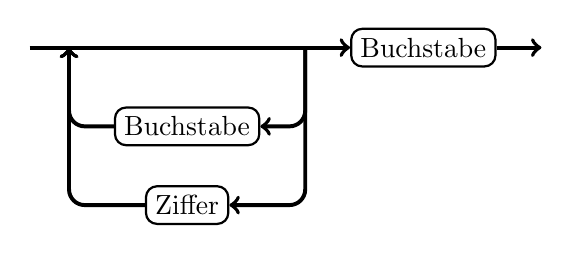
\begin{tikzpicture}
% \draw[help lines] (0,0) grid (7,2);
% \node at (0,3) {Bezeichner:};
%
\node (b1) [rounded corners,draw=black,thick] at (7,2) {\Snterm{Buchstabe}};
\node (b2) [rounded corners,draw=black,thick] at (4,1) {\Snterm{Buchstabe}};
\node (z)[rounded corners,draw=black,thick] at (4,0) {\Snterm{Ziffer}};
% \draw[decorate,thick] (0,0) -- (0,3) -- (3,3);
\draw [->,line width=0.5mm] (b1) -> (8.5,2);
\draw [->,line width=0.5mm] (2,2) -> (b1);
\draw [->,rounded corners=2mm,line width=0.5mm] (b2) -- (2.5,1) -> (2.5,2);
\draw [->,rounded corners=2mm,line width=0.5mm] (z) -- (2.5,0) -> (2.5,2);
\draw [->,rounded corners=2mm,line width=0.5mm] (5.5,2) -- (5.5,1) -> (b2);
\draw [->,rounded corners=2mm,line width=0.5mm] (5.5,2) -- (5.5,0) -> (z);
\end{tikzpicture}
\end{center}
\bigskip

Entsprechender NFA:

\begin{center}
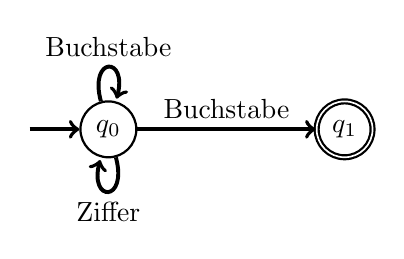
\begin{tikzpicture}
% \draw[help lines] (0,0) grid (7,2);
\node (s1) [circle,draw=black,thick] at (0,0) {$q_0$};
\node (s2) [double,circle,draw=black,thick] at (3,0) {$q_1$};
%
\path[->,line width=0.5mm](-1,0) edge (s1);
\path[->,line width=0.5mm](s1) edge node[above] {\Snterm{Buchstabe}} (s2);
\path[->,line width=0.5mm](s1) edge [loop above] node[above] {\Snterm{Buchstabe}} (s1);
\path[->,line width=0.5mm](s1) edge [loop below] node[below] {\Snterm{Ziffer}} (s1);
\end{tikzpicture}
\end{center}

\end{frame}


\begin{frame}\frametitle{Verallgemeinerte NFA-Übergangsfunktion}

Wie beim DFA können wir auch bei einem NFA $\Smach{M}=\tuple{Q,\Sigma,\delta,Q_0,F}$ eine erweiterte Übergangsfunktion 
definieren, die ganze Wörter \ghost{einliest.}
\medskip

Zuerst erweitern wir $\delta$ auf \alert{Mengen von Zuständen:}

\defbox{Für eine Zustandsmenge $R\subseteq Q$ und ein Terminalsymbol $\Sterm{a}$ sei
\[\delta(R,\Sterm{a})=\bigcup_{q\in R}\delta(q,\Sterm{a}).\]
}\pause

Dann erweitern wir $\delta$ von einzelnen Symbolen zu \alert{beliebigen \ghost{Wörtern:}}

\defbox{%Wir definieren eine Funktion $\delta: 2^Q\times \Sigma^* \to 2^Q$:\\
Für eine Zustandsmenge $R\subseteq Q$ und ein Wort $w\in\Sigma^*$ sei $\delta(R,w)$ die Menge aller Zustände,
die man erreichen kann, wenn man in einem Zustand aus $R$ beginnt und das Wort $w$ einliest, formal:
\begin{itemize}
\item $\delta(R,\epsilon)= R$
% \item $\delta(R,\Sterm{a})=\bigcup_{q\in R}\delta(q,\Sterm{a})$
\item $\delta(R,\Sterm{a}v)= \delta(\delta(R,\Sterm{a}),v)$
\end{itemize}

}

\end{frame}

\begin{frame}\frametitle{Beispiel}

\doodlebox{darkgreen}{%
\emph{Beispiel:}
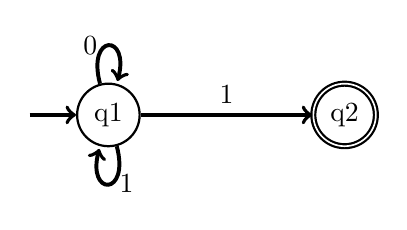
\begin{tikzpicture}[baseline={([yshift=-2ex]current bounding box.north)}]
% \draw[help lines] (0,0) grid (7,2);
\node (s1) [circle,draw=black,thick] at (0,0) {q1};
\node (s2) [double,circle,draw=black,thick] at (3,0) {q2};
%
\path[->,line width=0.5mm](-1,0) edge (s1);
\path[->,line width=0.5mm](s1) edge [loop above] node[left] {\Sterm{0}} (s1);
\path[->,line width=0.5mm](s1) edge [loop below] node[right] {\Sterm{1}} (s1);
\path[->,line width=0.5mm](s1) edge node[above] {\Sterm{1}} (s2);
\end{tikzpicture}%
\hspace{1cm}
\begin{minipage}[t]{3cm}
$\delta(q_1,\Sterm{0}) = \{q_1\}$\\
$\delta(q_1,\Sterm{1}) = \{q_1,q_2\}$\\
$\delta(q_2,\Sterm{0}) = \emptyset$\\
$\delta(q_2,\Sterm{1}) = \emptyset$
\end{minipage}
}

Die Menge der Startzustände ist $Q_0=\{q_1\}$.
\bigskip

Dann gilt:
\begin{align*}
\delta(Q_0,\Sterm{0}) &= \delta(q_1,\Sterm{0}) = \{q_1\}\\[1ex]
\delta(Q_0,\Sterm{1}) &= \delta(q_1,\Sterm{1}) = \{q_1,q_2\}\\[1ex]
\delta(Q_0,\Sterm{10}) &= \delta(\delta(Q_0,\Sterm{1}),\Sterm{0}) = \delta(\{q_1,q_2\},\Sterm{0})\\
	&= \delta(q_1,\Sterm{0})\cup  \delta(q_2,\Sterm{0}) = \{q_1\}\cup\emptyset =\{q_1\}\\[1ex]
\delta(Q_0,\Sterm{01}) &= \delta(\delta(Q_0,\Sterm{0}),\Sterm{1}) = \delta(\{q_1\},\Sterm{1}) = \{q_1,q_2\}
\end{align*}

\end{frame}

\begin{frame}\frametitle{Sprache eines NFA (2. Version)}

Die erweiterte Übergangsfunktion hilft bei der Definition der Sprache, die ein NFA akzeptiert:
\bigskip

\defbox{
Die \redalert{Sprache eines NFA} $\Smach{M}=\tuple{Q,\Sigma,\delta,Q_0,F}$ ist die Menge\\[1ex]
\narrowcentering{$\Slang{L}(\Smach{M}) = \{w\in\Sigma^*\mid \delta(Q_0,w)\cap F \neq \emptyset\}$}
}

Die Bedingung \alert{"`$\delta(Q_0,w)\cap F \neq \emptyset$"'} bedeutet:\\[1ex] \alert{"`mindestens einer der Zustände, die man durch Einlesen von $w$ von einem Startzustand aus erreichen kann, ist ein Endzustand."'}
% \medskip
% \redalert{das ist gleichbedeutend mit:}
% \medskip
%  \alert{"`es gibt eine Folge von Zuständen, die man durch nichtdeterministische."'}

\bigskip

\emph{Behauptung:} Diese Variante stimmt mit der vorherigen (mit akzeptierenden Läufen) überein.

% 
% \doodlebox{darkgreen}{%
% Beispiel:
% \begin{tikzpicture}[baseline={([yshift=-2ex]current bounding box.north)}]
% % \draw[help lines] (0,0) grid (7,2);
% \node (s1) [circle,draw=black,thick] at (0,0) {q1};
% \node (s2) [double,circle,draw=black,thick] at (3,0) {q2};
% %
% \path[->,line width=0.5mm](-1,0) edge (s1);
% \path[->,line width=0.5mm](s1) edge [loop above] node[left] {\Sterm{0}} (s1);
% \path[->,line width=0.5mm](s1) edge [loop below] node[right] {\Sterm{1}} (s1);
% \path[->,line width=0.5mm](s1) edge node[above] {\Sterm{1}} (s2);
% \end{tikzpicture}%
% \hspace{1cm}
% \begin{minipage}[t]{3cm}
% ~\\
% $\Slang{L}(\Smach{M})= \{\Sterm{0},\Sterm{1}\}^* \circ \{\Sterm{1}\}$\\
% ~\\
% ~
% \end{minipage}
% }

\end{frame}

\begin{frame}[t]\frametitle{Äquivalenz der Sprachdefinitionen für NFAs}

Sei $\Smach{M}=\tuple{Q,\Sigma,\delta,Q_0,F}$ NFA und $w=\sigma_1\cdots\sigma_n\in\Sigma^*$ ein Wort.\\[1ex]

\emph{Behauptung:} Es gibt einen akzeptierenden Lauf für $w$ genau dann wenn
$\delta(Q_0,w)\cap F \neq \emptyset$.\\[1ex]\pause

\emph{Beweis "`$\Rightarrow$"':}
Angenommen es gibt einen akzeptierenden Lauf $q_0\ldots q_n$ für $w$.\pause
\begin{itemize}
\item Dann ist $q_n\in F$.\pause
\item Wir behaupten $q_n\in \delta(Q_0,w)$ \textcolor{devilscss}{(damit folgt $\delta(Q_0,w)\cap F \neq \emptyset$)}\pause
\item Wir zeigen die stärkere Behauptung $q_i\in \delta(Q_0,\sigma_1\cdots\sigma_i)$ für alle $0\leq i\leq n$
mittels Induktion über $|w|$\pause:
\begin{itemize}
\item Induktionsanfang: Für $i=0$ gilt $q_0\in Q_0 = \delta(Q_0,\epsilon)$\pause
\item Induktionshypothese: die Behauptung gelte für $i$\pause
\item Induktionsschritt: für $i+1$ gilt:\\
	$q_i\in \delta(Q_0,\sigma_1\cdots\sigma_i)$ \textcolor{devilscss}{(Induktionshypothese)}\\
	$q_{i+1}\in\delta(q_i,\sigma_{i+1})$ \textcolor{devilscss}{(laut Definition eines Laufs)}\\
	$q_{i+1}\in\delta(\delta(Q_0,\sigma_1\cdots\sigma_i),\sigma_{i+1})=\delta(Q_0,\sigma_1\cdots\sigma_i\sigma_{i+1})$
\end{itemize}
\end{itemize}
\end{frame}

\begin{frame}[t]\frametitle{Äquivalenz der Sprachdefinitionen für NFAs}

Sei $\Smach{M}=\tuple{Q,\Sigma,\delta,Q_0,F}$ NFA und $w=\sigma_1\cdots\sigma_n\in\Sigma^*$ ein Wort.\\[1ex]

\emph{Behauptung:} Es gibt einen akzeptierenden Lauf für $w$ genau dann wenn
$\delta(Q_0,w)\cap F \neq \emptyset$.\\[1ex]

\emph{Beweis "`$\Leftarrow$"':}
Angenommen $\delta(Q_0,w)\cap F \neq \emptyset$.\pause
\begin{itemize}
\item Wir ermitteln einen akzeptierenden Lauf $q_0\ldots q_n$ für $w$\pause
\item Dazu gehen wir rückwärts vor:
\begin{itemize}
\item Wähle $q_n\in F\cap\delta(Q_0,w)$
\item Für alle $i=n,\ldots,1$:\\
Wähle $q_{i-1}\in\delta(Q_0,\sigma_1\cdots\sigma_{i-1})$, so dass $q_i\in\delta(q_{i-1},\sigma_i) $
\end{itemize}\pause
\item Dies ist ein Lauf, da $q_0\in\delta(Q_0,\epsilon)=Q_0$ und alle Übergänge erlaubt sind.
\item Es ist ein akzeptierender Lauf, da $q_n\in F$.\qed
\end{itemize}
\end{frame}

% Potenzmengenkonstruktion

\sectionSlide{NFA vs. DFA}

\begin{frame}\frametitle{Vergleich DFA -- NFA}

Offensichtlich sind NFAs allgemeiner als DFAs:

\theobox{\emph{Satz:} Jeder DFA kann als NFA aufgefasst werden. Daher wird jede von einem DFA akzeptierbare Sprache auch von einen NFA akzeptiert.}

\emph{Beweis:} Für jeden DFA  $\Smach{M}=\tuple{Q,\Sigma,\delta,q_0,F}$ gibt es
einen entsprechenden NFA $\Smach{M}'=\tuple{Q,\Sigma,\delta_{\textsf{NFA}},\{q_0\},F}$
mit $\delta_{\textsf{NFA}}(q,\Sterm{a}) = \{\delta(q,\Sterm{a})\}$.\qed
\bigskip
\pause

Die Umkehrung dieses Satzes gilt allerdings auch:
\theobox{\emph{Satz:} Jede von einem NFA akzeptierbare Sprache wird auch von einen DFA akzeptiert.}

In diesem Sinne sind NFA nicht ausdrucksstärker als DFA -- wie kann das sein?

\end{frame}

\begin{frame}\frametitle{NFAs als DFAs -- Idee}

Die verallgemeinerte NFA-Übergangsfunktion bildet \redalert{Mengen von Zuständen} auf
\redalert{Mengen von Zuständen} ab:
\[\delta(R,\Sterm{a})=\bigcup_{q\in R}\delta(q,\Sterm{a}).\]
% \medskip

\alert{"`Wenn der Automat in einem der Zustände $R$ ist und $\Sterm{a}$ liest, so ist er anschließend in einem der Zustände der Menge $\delta(R,\Sterm{a})$."'}
\medskip

Dieser Übergang zwischen Mengen möglicher Zustände ist an sich deterministisch.
\bigskip

$\leadsto$ wir können einen NFA deterministisch simulieren, indem wir die Menge der möglichen Zustände berechnen

\end{frame}

\begin{frame}\frametitle{Die Potenzmengenkonstruktion}

\defbox{Für einen NFA $\Smach{M}=\tuple{Q,\Sigma,\delta,Q_0,F}$ definieren wir den \redalert{Potenzmengen-DFA} 
$\Smach{M}_{\textsf{DFA}}=\tuple{Q_{\textsf{DFA}},\Sigma,\delta_{\textsf{DFA}},q_0,F_{\textsf{DFA}}}$
wie folgt:%
\begin{itemize}
\item $Q_{\textsf{DFA}}=2^Q$ (Potenzmenge von $Q$)
\item $\delta_{\textsf{DFA}}(R,\Sterm{a})=\bigcup_{q\in R}\delta(q,\Sterm{a})$
\item $q_0=Q_0$
\item $F_{\textsf{DFA}}=\{R\in 2^Q\mid R\cap F \neq \emptyset\}$
\end{itemize}
}
\smallskip

\theobox{\emph{Satz (Rabin/Scott):} $\Slang{L}(\Smach{M}) = \Slang{L}(\Smach{M}_{\textsf{DFA}})$}

(Beweis später)\hspace{8.1cm}\ghost{\raisebox{-1.7cm}{\includegraphics[height=2cm]{images/Rabin-Scott}~\rotatebox{90}{\tiny Andrej Bauer, CC-BY-SA 2.5}}}
\vspace{1.5cm}

\hspace{10.1cm} \ghost{{\tiny Michael Oser Rabin~~~~~~Dana Scott}}

% 
% Beispiel:
% 
% \begin{tikzpicture}[baseline={([yshift=-2ex]current bounding box.north)}]
% % \draw[help lines] (0,0) grid (7,2);
% \node (s1) [circle,draw=black,thick] at (0,0) {q1};
% \node (s2) [double,circle,draw=black,thick] at (3,0) {q2};
% %
% \path[->,line width=0.5mm](-1,0) edge (s1);
% \path[->,line width=0.5mm](s1) edge [loop above] node[left] {\Sterm{0}} (s1);
% \path[->,line width=0.5mm](s1) edge [loop below] node[right] {\Sterm{1}} (s1);
% \path[->,line width=0.5mm](s1) edge node[above] {\Sterm{1}} (s2);
% \end{tikzpicture}\hfill
% %
% \begin{tikzpicture}[baseline={([yshift=-2ex]current bounding box.north)}]
% % \draw[help lines] (0,0) grid (7,2);
% \node (s1) [circle,draw=black,thick] at (0,0) {$\{q1\}$};
% \node (s12) [double,circle,draw=black,thick] at (3,0) {$\{q1,q2\}$};
% \node (s0) [circle,draw=black,thick] at (0,-1.7) {$\emptyset$};
% \node (s2) [double,circle,draw=black,thick] at (3,-1.7) {$\{q2\}$};
% %
% \path[->,line width=0.5mm](-1,0) edge (s1);
% \path[->,line width=0.5mm](s1) edge [loop above] node[left] {\Sterm{0}} (s1);
% \path[->,line width=0.5mm](s12) edge [loop above] node[left] {\Sterm{1}} (s12);
% % \path[->,line width=0.5mm](s1) edge [loop below] node[right] {\Sterm{1}} (s1);
% % \path[->,line width=0.5mm](s1) edge node[above] {\Sterm{1}} (s2);
% \end{tikzpicture}



\end{frame}

\begin{frame}\frametitle{Beispiel Potenzmengenkonstruktion}

\begin{minipage}{5cm}
\begin{tikzpicture}[baseline={([yshift=-2ex]current bounding box.north)}]
% \draw[help lines] (0,0) grid (7,2);
\node (s1) [circle,draw=black,thick,onslide={<5,6,9,10>{fill=strongyellow}}] at (0,0) {$q_0$};
\node (s2) [double,circle,draw=black,thick,onslide={<3,7,8,9,10>{fill=strongyellow}}] at (3,0) {$q_1$};
%
\path[->,line width=0.5mm,onslide={<4>{dashed,darkred}}](0,1) edge (s1);
\path[->,line width=0.5mm,onslide={<4>{dashed,darkred}}](3,1) edge (s2);
\path[->,line width=0.5mm,onslide={<6,10>{dashed,darkred}}](s1) edge [loop below] node[left] {\Sterm{1}} (s1);
\path[->,line width=0.5mm,bend left,onslide={<6,10>{dashed,darkred}}](s1) edge node[above] {\Sterm{1}} (s2);
\path[->,line width=0.5mm,bend left,onslide={<7,9>{dashed,darkred}}](s2) edge node[above] {\Sterm{0}} (s1);
% \path[->,line width=0.5mm](s1) edge node[above] {\Sterm{1}} (s2);
\end{tikzpicture}
\bigskip

\begin{tikzpicture}[baseline={([yshift=-2ex]current bounding box.north)}]
% \draw[help lines] (0,0) grid (7,2);
\onslide<2->{\node (s12) [rectangle,rounded corners=1.5ex,onslide={<3->{double}},draw=black,thick] at (0,0) {$\{q_0,q_1\}$};}
\onslide<2->{\node (s1) [rectangle,rounded corners=1.5ex,draw=black,thick] at (3,0) {$\{q_0\}$};}
\onslide<2->{\node (s2) [onslide={<3->{double}},rectangle,rounded corners=1.5ex,draw=black,thick] at (3,-2) {$\{q_1\}$};}
\onslide<2->{\node (s0) [circle,draw=black,thick] at (0,-2) {$\emptyset$};}
%,onslide={<1>{color=white}}
\onslide<4->{\path[->,line width=0.5mm,onslide={<4>{dashed,darkred}}](0,1) edge (s12);}
\onslide<10->{\path[->,line width=0.5mm,onslide={<10>{dashed,darkred}}](s12) edge [loop left] node[left] {\Sterm{1}} (s12);}
\onslide<9->{\path[->,line width=0.5mm,bend left,onslide={<9>{dashed,darkred}}](s12) edge node[above] {\Sterm{0}} (s1);}
\onslide<6->{\path[->,line width=0.5mm,bend left,onslide={<6>{dashed,darkred}}](s1) edge node[above] {\Sterm{1}} (s12);}
\onslide<7->{\path[->,line width=0.5mm,onslide={<7>{dashed,darkred}}](s2) edge node[left] {\Sterm{0}} (s1);}
\onslide<5->{\path[->,line width=0.5mm,onslide={<5>{dashed,darkred}}](s1) edge node[below] {\Sterm{0}} (s0);}
\onslide<8->{\path[->,line width=0.5mm,onslide={<8>{dashed,darkred}}](s2) edge node[below] {\Sterm{1}} (s0);}
\onslide<11->{\path[->,line width=0.5mm,onslide={<11>{dashed,darkred}}](s0) edge [loop left] node[left] {\Sterm{0},\Sterm{1}} (s0);}
\end{tikzpicture}
\end{minipage}\hfill
\begin{minipage}{4cm}
\onslide<5->{$\delta_{\textsf{DFA}}(\{q_0\},\Sterm{0}) = \emptyset$}\\
\onslide<6->{$\delta_{\textsf{DFA}}(\{q_0\},\Sterm{1}) = \{q_0,q_1\}$}\\
\onslide<7->{$\delta_{\textsf{DFA}}(\{q_1\},\Sterm{0}) = \{q_0\}$}\\
\onslide<8->{$\delta_{\textsf{DFA}}(\{q_1\},\Sterm{1}) = \emptyset$}\\
\onslide<9->{$\delta_{\textsf{DFA}}(\{q_0,q_1\},\Sterm{0}) = \{q_0\}$}\\
\onslide<10->{$\delta_{\textsf{DFA}}(\{q_0,q_1\},\Sterm{1}) = \{q_0,q_1\}$}\\
\onslide<11->{$\delta_{\textsf{DFA}}(\emptyset,\Sterm{0}) = \emptyset$}\\
\onslide<11->{$\delta_{\textsf{DFA}}(\emptyset,\Sterm{1}) = \emptyset$}
\bigskip

\onslide<12->{Erkannte Sprache:\\ $\{\Sterm{1}\}^* \circ (\{\Sterm{0}\}\circ \{\Sterm{1}\}^+)^*$}
\end{minipage}
\end{frame}

\begin{frame}\frametitle{Vereinfachung Potenzmengenkonstruktion}

Der Automat aus dem vorherigen Beispiel kann vereinfacht \ghost{werden:}

\begin{tikzpicture}[baseline={([yshift=-2ex]current bounding box.north)}]
% \draw[help lines] (0,0) grid (7,2);
\node (s12) [double,rectangle,rounded corners=1.5ex,draw=black,thick] at (0,0) {$\{q_0,q_1\}$};
\node (s1) [rectangle,rounded corners=1.5ex,draw=black,thick] at (3,0) {$\{q_0\}$};
\onslide<-2>{\node (s2) [double,rectangle,rounded corners=1.5ex,draw=black,thick,onslide={<2>{draw=darkred}}] at (3,-2) {$\{q_1\}$};}
\onslide<-4>{\node (s0) [circle,draw=black,thick,onslide={<4>{draw=darkred}}] at (0,-2) {$\emptyset$};}
%,onslide={<1>{color=white}}
\path[->,line width=0.5mm](0,1) edge (s12);
\path[->,line width=0.5mm](s12) edge [loop left] node[left] {\Sterm{1}} (s12);
\path[->,line width=0.5mm,bend left](s12) edge node[above] {\Sterm{0}} (s1);
\path[->,line width=0.5mm,bend left](s1) edge node[above] {\Sterm{1}} (s12);
\onslide<-2>{\path[->,line width=0.5mm,onslide={<2>{dashed,darkred}}](s2) edge node[left] {\Sterm{0}} (s1);}
\onslide<-4>{\path[->,line width=0.5mm,onslide={<4>{dashed,darkred}}](s1) edge node[below] {\Sterm{0}} (s0);}
\onslide<-2>{\path[->,line width=0.5mm,onslide={<2>{dashed,darkred}}](s2) edge node[below] {\Sterm{1}} (s0);}
\onslide<-4>{\path[->,line width=0.5mm,onslide={<4>{dashed,darkred}}](s0) edge [loop left] node[left] {\Sterm{0},\Sterm{1}} (s0);}
\end{tikzpicture}

\pause
\begin{itemize}
\item Zustand $\{q_1\}$ ist unerreichbar\pause\pause
\item Zustand $\emptyset$ kann nicht verlassen werden (irrelevant für akzeptierende Läufe)\pause
\end{itemize}

\end{frame}

\begin{frame}\frametitle{Potenzmengenkonstruktion "`on the fly"'}

Vermeidung unnötiger Zustände durch schrittweise Konstruktion vom Startzustand:
\medskip

\begin{minipage}{5cm}%
\begin{tikzpicture}[baseline={([yshift=-2ex]current bounding box.north)}]
% \draw[help lines] (0,0) grid (7,2);
\node (s1) [double,circle,draw=black,thick] at (0,0) {$q_1$};
\node (s2) [circle,draw=black,thick] at (3,0) {$q_2$};
\node (s3) [circle,draw=black,thick] at (0,-2) {$q_3$};
%
\path[->,line width=0.5mm,onslide={<2>{dashed,darkred}}](0,1) edge (s1);
\path[->,line width=0.5mm,onslide={<2>{dashed,darkred}}](3,1) edge (s2);
\path[->,line width=0.5mm,onslide={<3,7>{dashed,darkred}}](s1) edge node[above] {\Sterm{0}} (s2);
\path[->,line width=0.5mm,bend left,onslide={<3,4>{dashed,darkred}}](s2) edge node[above] {\Sterm{0}} (s3);
\path[->,line width=0.5mm,bend left,onslide={<3,7>{dashed,darkred}}](s1) edge node[left] {\Sterm{0}} (s3);
\path[->,line width=0.5mm,bend left,onslide={<5,6,8>{dashed,darkred}}](s3) edge node[left] {\Sterm{1}} (s1);
\path[->,line width=0.5mm,onslide={<5,6,8>{dashed,darkred}}](s3) edge [loop below] node[below] {\Sterm{1}} (s3);
\end{tikzpicture}
\bigskip

\onslide<12->{
\begin{itemize}
\item Erreichbarer Teil spart drei Zustände ein
\item Zustand $\emptyset$ wie zuvor unnötig
\end{itemize}
}
\end{minipage}
%
\begin{minipage}{4cm}
\begin{tikzpicture}[baseline={([yshift=-2ex]current bounding box.north)}]
% \draw[help lines] (0,0) grid (7,2);
\onslide<2->{\node (s12) [double,rectangle,rounded corners=1.5ex,draw=black,thick,onslide={<2>{fill=strongyellow}}] at (0,0) {~$\{q_1,q_2\}$~\mbox{}};}
\onslide<9->{\node (s0) [circle,draw=black,thick,onslide={<9>{fill=strongyellow}}] at (3,0) {$\emptyset$};}
\onslide<3->{\node (s32) [rectangle,rounded corners=1.5ex,draw=black,thick,onslide={<3>{fill=strongyellow}}] at (0,-2) {~$\{q_2,q_3\}$~\mbox{}};}
\onslide<4->{\node (s3) [rectangle,rounded corners=1.5ex,draw=black,thick,onslide={<4>{fill=strongyellow}}] at (3,-2) {~$\{q_3\}$~\mbox{}};}
\onslide<5->{\node (s31) [double,rectangle,rounded corners=1.5ex,draw=black,thick,onslide={<5>{fill=strongyellow}}] at (1.5,-4) {~$\{q_1,q_3\}$~\mbox{}};}
%
\onslide<2->{\path[->,line width=0.5mm,onslide={<2>{dashed,darkred}}](0,1) edge (s12);}
\onslide<10->{\path[->,line width=0.5mm,onslide={<10>{dashed,darkred}}](s12) edge node[above] {\Sterm{1}} (s0);}
\onslide<11->{\path[->,line width=0.5mm,onslide={<11>{dashed,darkred}}](s0) edge [loop above] node[above] {\Sterm{0},\Sterm{1}} (s0);}
\onslide<3->{\path[->,line width=0.5mm,onslide={<3>{dashed,darkred}}](s12) edge node[right] {\Sterm{0}} (s32);}
\onslide<4->{\path[->,line width=0.5mm,onslide={<4>{dashed,darkred}}](s32) edge node[above] {\Sterm{0}} (s3);}
\onslide<9->{\path[->,line width=0.5mm,onslide={<9>{dashed,darkred}}](s3) edge node[right] {\Sterm{0}} (s0);}
\onslide<5->{\path[->,line width=0.5mm,onslide={<5>{dashed,darkred}}](s3) edge node[above] {\Sterm{1}} (s31);}
\onslide<8->{\path[->,line width=0.5mm,onslide={<8>{dashed,darkred}}](s32) edge node[above] {\Sterm{1}} (s31);}
\onslide<7->{\path[->,line width=0.5mm,bend left,onslide={<7>{dashed,darkred}}](s31) edge node[left] {\Sterm{0}} (s32);}
\onslide<6->{\path[->,line width=0.5mm,onslide={<6>{dashed,darkred}}](s31) edge [loop right] node[right] {\Sterm{1}} (s31);}
\end{tikzpicture}
\end{minipage}


\end{frame}


\begin{frame}[t]\frametitle{Potenzmengenkonstruktion: Korrektheit}

\theobox{\emph{Satz (Rabin/Scott):} $\Slang{L}(\Smach{M}) = \Slang{L}(\Smach{M}_{\textsf{DFA}})$}

\emph{Beweis:} Wir nutzen die Korrespondenz der verallgemeinerten Übergangsfunktionen aus. Zuerst zeigen wir,
dass für jedes Wort $w\in\Sigma^*$ und jede Zustandsmenge $R$ gilt: $\delta_{\textsf{DFA}}(R,w) = \delta(R,w)$.\pause
\medskip

\alert{Induktionsanfang:}
\begin{enumerate}[(1)]
\item $\delta_{\textsf{DFA}}(R,\epsilon) = R = \delta(R,\epsilon)$\pause
\item $\delta_{\textsf{DFA}}(R,\Sterm{a}) = \bigcup_{q\in R}\delta(q,\Sterm{a}) = \delta(R,\Sterm{a})$\pause
\end{enumerate}\medskip

\alert{Induktionshypothese:} $\delta_{\textsf{DFA}}(R,v) = \delta(R,v)$ für Wörter $v$ der Länge $\ell$\\[1ex]
\alert{Induktionsschritt:} wir zeigen $\delta_{\textsf{DFA}}(R,\Sterm{a}v) = \delta(R,\Sterm{a}v)$ ein beliebiges Wort $\Sterm{a}v$ der \ghost{Länge $\ell+1$}
\begin{enumerate}[(3)]
\item $\delta_{\textsf{DFA}}(R,\Sterm{a}v) = \delta_{\textsf{DFA}}(\delta_{\textsf{DFA}}(R,\Sterm{a}),v)$\\\pause
\hspace{1.58cm}${}= \delta_{\textsf{DFA}}(\delta(R,\Sterm{a}),v)$ \hspace{1cm}(wegen (2))\\\pause
\hspace{1.58cm}${}= \delta(\delta(R,\Sterm{a}),v)$ \hspace{1.45cm}(Induktionshypothese)\\\pause
\hspace{1.58cm}${}= \delta(R,\Sterm{a}v)$
\end{enumerate}

\end{frame}

\begin{frame}[t]\frametitle{Potenzmengenkonstruktion: Korrektheit (2)}

\theobox{\emph{Satz (Rabin/Scott):} $\Slang{L}(\Smach{M}) = \Slang{L}(\Smach{M}_{\textsf{DFA}})$}

\emph{Beweis (Fortsetzung):} Wir haben gezeigt: $\delta_{\textsf{DFA}}(R,w) = \delta(R,w)$.\pause
\medskip

Damit ergibt sich, für beliebige Wörter $w\in\Sigma^*$:\medskip

\begin{tabular}{l@{~~~ gdw. ~~~}l}
$w\in \Slang{L}(\Smach{M})$ & \pause$\delta(Q_0,w)\cap F \neq \emptyset$ \\\pause
	& $\delta_{\textsf{DFA}}(Q_0,w)\cap F \neq \emptyset$ \\\pause
	& $\delta_{\textsf{DFA}}(Q_0,w)\in F_{\textsf{DFA}}$ \\\pause
	& $w\in \Slang{L}(\Smach{M}_{\textsf{DFA}})$
\end{tabular}

\qed

\end{frame}

\begin{frame}\frametitle{Größenvergleich}

Der DFA eines NFA hat $2^{|Q|}$ -- also exponentiell viele -- Zustände.\\
Auch "`on the fly"' lässt sich das im Allgemeinen nicht vermeiden.
\medskip

\emph{Beispiel:} "`Wörter mit \Sterm{1} an drittletzter Stelle"'

\narrowcentering{%
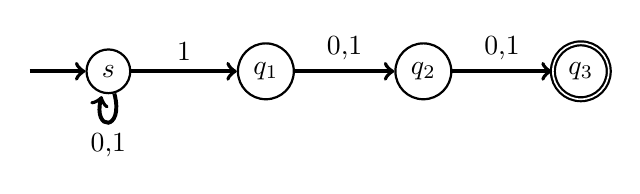
\begin{tikzpicture}[baseline={([yshift=-2ex]current bounding box.north)}]
% \draw[help lines] (0,0) grid (7,2);
\node (sx) [circle,draw=black,thick] at (0,0) {$s$};
\node (s1) [circle,draw=black,thick] at (2,0) {$q_1$};
\node (s2) [circle,draw=black,thick] at (4,0) {$q_2$};
\node (s3) [double,circle,draw=black,thick] at (6,0) {$q_3$};
%
\path[->,line width=0.5mm](-1,0) edge (sx);
\path[->,line width=0.5mm](sx) edge [loop below] node[below] {\Sterm{0},\Sterm{1}} (sx);
\path[->,line width=0.5mm](sx) edge node[above] {\Sterm{1}} (s1);
\path[->,line width=0.5mm](s1) edge node[above] {\Sterm{0},\Sterm{1}} (s2);
\path[->,line width=0.5mm](s2) edge node[above] {\Sterm{0},\Sterm{1}} (s3);
\end{tikzpicture}}
\vspace{-5mm}\pause

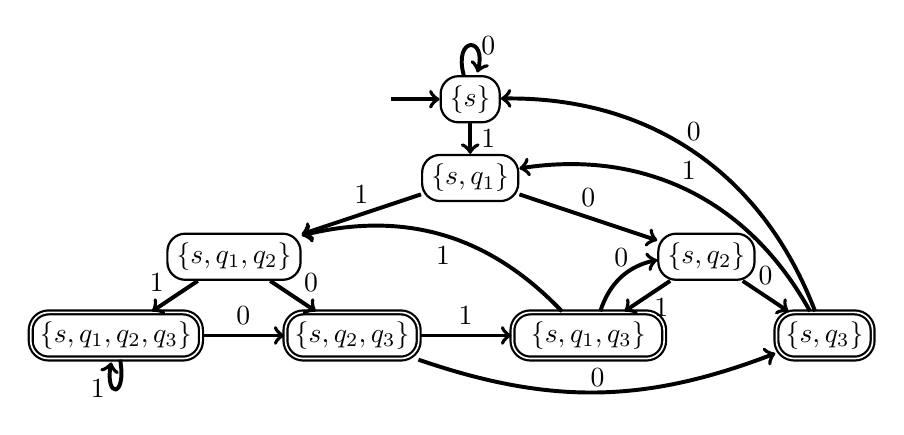
\begin{tikzpicture}[baseline={([yshift=-2ex]current bounding box.north)}]
% \draw[help lines] (0,0) grid (7,2);
\node (sx) [rectangle,rounded corners=1.5ex,draw=black,thick] at (0,0) {$\{s\}$};
\node (sx1) [rectangle,rounded corners=1.5ex,draw=black,thick] at (0,-1) {$\{s,q_1\}$};
\node (sx2) [rectangle,rounded corners=1.5ex,draw=black,thick] at (3,-2) {$\{s,q_2\}$};
\node (sx12) [rectangle,rounded corners=1.5ex,draw=black,thick] at (-3,-2) {$\{s,q_1,q_2\}$};
\node (sx3) [rectangle,rounded corners=1.5ex,double,draw=black,thick] at (4.5,-3) {$\{s,q_3\}$};
\node (sx13) [rectangle,rounded corners=1.5ex,double,draw=black,thick] at (1.5,-3) {$~\{s,q_1,q_3\}~$};
\node (sx23) [rectangle,rounded corners=1.5ex,double,draw=black,thick] at (-1.5,-3) {$\{s,q_2,q_3\}$};
\node (sx123) [rectangle,rounded corners=1.5ex,double,draw=black,thick] at (-4.5,-3) {$\{s,q_1,q_2,q_3\}$};
%
\path[->,line width=0.5mm](-1,0) edge (sx);
\path[->,line width=0.5mm](sx) edge [loop above] node[right] {\Sterm{0}} (sx);
\path[->,line width=0.5mm](sx) edge node[right] {\Sterm{1}} (sx1);
%
\path[->,line width=0.5mm](sx1) edge node[above] {\Sterm{0}} (sx2);
\path[->,line width=0.5mm](sx2) edge node[above] {\Sterm{0}} (sx3);
%
\path[->,line width=0.5mm](sx2) edge node[below, xshift=5pt, yshift=3pt] {\Sterm{1}} (sx13);
%
\path[->,line width=0.5mm](sx1) edge node[above] {\Sterm{1}} (sx12);
\path[->,line width=0.5mm](sx12) edge node[right, yshift=5pt] {\Sterm{0}} (sx23);
%
\path[->,line width=0.5mm](sx12) edge node[left, yshift=5pt] {\Sterm{1}} (sx123);
%
%
\path[->,line width=0.5mm](sx123) edge [in=260,out=280,loop] node[left] {\Sterm{1}} (sx123);
\path[->,line width=0.5mm](sx123) edge node[above] {\Sterm{0}} (sx23);
%
\path[->,line width=0.5mm](sx23) edge node[above] {\Sterm{1}} (sx13);
\path[->,line width=0.5mm,bend right=20](sx23) edge node[above, yshift=-2pt] {\Sterm{0}} (sx3);
%
\path[->,line width=0.5mm,bend right](sx13) edge node[below] {\Sterm{1}} (sx12);
\path[->,line width=0.5mm,bend left](sx13) edge node[above] {\Sterm{0}} (sx2);
%
\path[->,line width=0.5mm,bend right=35](sx3) edge node[above] {\Sterm{0}} (sx);
\path[->,line width=0.5mm,bend right=35](sx3) edge node[above] {\Sterm{1}} (sx1);
%
% \path[->,line width=0.5mm](sx) edge [loop above] node[above] {\Sterm{0},\Sterm{1}} (sx);
% \path[->,line width=0.5mm](sx) edge node[above] {\Sterm{1}} (s1);
% \path[->,line width=0.5mm](s1) edge node[above] {\Sterm{0},\Sterm{1}} (s2);
% \path[->,line width=0.5mm](s2) edge node[above] {\Sterm{0},\Sterm{1}} (s3);
\end{tikzpicture}


\end{frame}

\begin{frame}\frametitle{Größenvergleich (2)}

Allgemein kann man für jede Zahl $n\geq 1$ die Sprache $\Slang{L}_n= \{\Sterm{0},\Sterm{1}\}^* \Sterm{1} \{\Sterm{0},\Sterm{1}\}^{n-1} $ betrachten ("`Wörter mit \Sterm{1} an $n$-letzter Stelle"')
\medskip

Es gilt:
\begin{itemize}
\item Es gibt einen NFA mit $n+1$ Zuständen, der $\Slang{L}_n$ erkennt.
\item Jeder DFA, der $\Slang{L}_n$ erkennt, hat mindestens $2^n$ Zustände.
\end{itemize}

\bigskip

\emph{Schlussfolgerung:}\\
\alert{NFAs können exponentiell kompakter sein als äquivalente DFAs.}

\end{frame}


\begin{frame}[fragile]\frametitle{Darstellungen von Typ-3-Sprachen}

% Diagram mit Uebersetzungen reg Gram, DFA, NFA
% TODO Maybe add overlays

\begin{tikzpicture}[
	decoration=penciline, decorate,
	node distance = 7mm and 9mm,
	mybox/.style args = {#1/#2}{
		draw=#1,% line color
		fill=#2,% fill color
% 		rounded corners,
		thick,
		text width=26mm, minimum height=12mm, inner sep=1mm, 
		align=flush center
	},
	myboxlabel/.style args = {}{
		draw=devilscss,% line color
		fill=strongyellow!40,% fill color
% 		rounded corners,
		thick,
		text width=21mm, minimum height=10mm, inner sep=1.5mm, 
		align=flush center
	},
	myarrow/.style args = {#1}{
		line width=0.8mm,
		draw=#1,%line color
		%-{Triangle[length=2.8mm,width=4mm,fill=#1]},
		->,
		shorten >=0.5mm, shorten <=0.1mm
	}
]
\pgfmathsetseed{7729}
% \draw[help lines] (0,0) grid (5,5);
\node (reg) [decorate,mybox=black/cyan!40] at (3,-0.6) {reguläre Grammatik};
\node (dfa) [decorate,mybox=black/cyan!40] at (0,-4) {DFA};
\node (nfa) [decorate,mybox=black/cyan!40] at (6,-4) {NFA};
%
\path[myarrow=devilscss,bend left=20](dfa) edge (reg.180);
\node (dfareglabel) [decorate,myboxlabel=,text width=19mm] at (-0.4,-0.7) {"`$q_1 \stackrel{\Sterm{a}}{\to} q_2$"' $\leadsto$ "`$q_1\to\Sterm{a}q_2$"'};
%
% \path[myarrow=devilscss,-,bend left=20](reg.0) edge[->] (nfa);
% \node (regnfalabel) [decorate,myboxlabel=] at (7.2,-2.1) {"`$q_1\to\Sterm{a}q_2$"' $\leadsto$ "`$q_1 \stackrel{\Sterm{a}}{\to} q_2$"'};
%
\draw[myarrow=devilscss](dfa.10)--(nfa.170);
\node (dfanfalabel) [decorate,myboxlabel=] at (3,-3.0) {\footnotesize DFAs sind spezielle NFAs};
%
\draw[myarrow=devilscss](nfa.190)--(dfa.350);
\node (nfadfalabel) [decorate,myboxlabel=] at (3,-5.0) {\footnotesize Potenzmengen\-konstruktion};
%
\node (sd) [decorate,mybox=black/cyan!40,text width=14mm, minimum height=10mm] at (6,-6.5) {\footnotesize Syntax\-diagramm};
\draw[myarrow=devilscss,<->](sd)--(nfa);
\node (sdnfalabel) [decorate,myboxlabel=, minimum height=0mm,inner sep=1.0mm,text width=10mm] at (6.9,-5.3) {\footnotesize dualer Graph};
\end{tikzpicture}

\end{frame}


\begin{frame}\frametitle{Von regulären Grammatiken zu NFAs}
% Direkt zur Definition; Idee wurde schon motiviert und kann bei Wiederholung genannt werden
% NFA fuer G heisst $\Smach{M}_G$

\theobox{
\emph{Satz:} Die Klasse der Sprachen, die durch DFAs oder NFAs erkannt werden können, ist genau die Klasse
der regulären Sprachen.
}

\emph{Beweis:} Wir können nun die noch fehlende Richtung dieser Behauptung zeigen:\\[0.5ex]
Für jede reguläre Grammatik $G$ gibt es einen NFA $\Smach{M}_G$, welcher die selbe Sprache akzeptiert (d.h., $\Slang{L}(G)=\Slang{L}(\Smach{M}_G)$).\smallskip\pause

\codebox{Für $G=\tuple{V,\Sigma,P,\Snterm{S}}$ ergibt sich $\Smach{M}_G=\tuple{Q,\Sigma,\delta,Q_0,F}$ wie folgt:
\begin{itemize}
\item $Q\defeq V\cup\{q_f\}$\pause
\item $Q_0\defeq \{\Snterm{S}\}$\pause
\item $F\defeq \{q_f\}\cup \{\Snterm{A}\in V\mid {\Snterm{A}\to\epsilon} \in P\}$\pause 
\item $\delta(\Snterm{A},\Sterm{c})\defeq\{\Snterm{B}\mid {\Snterm{A}\to\Sterm{c}\Snterm{B}}\in P\} \cup \{q_f\mid {\Snterm{A}\to\Sterm{c}}\in P\}$
\end{itemize}
}

\end{frame}

\begin{frame}\frametitle{Beispiel}
%notfalls einfach on CB Folie 10/25 18ff

Wir betrachten eine reguläre Grammatik mit den folgenden sechs Regeln:
%
\begin{align*}
\Snterm{S} &\to \Sterm{1} \mid \Sterm{0}\Snterm{A}\\
\Snterm{A} &\to \Sterm{0}\mid \Sterm{1} \mid \Sterm{1}\Snterm{A} \mid \epsilon
\end{align*}

Entsprechender NFA:

\narrowcentering{%
\begin{tikzpicture}[baseline={([yshift=-2ex]current bounding box.north)}]
% \draw[help lines] (0,0) grid (7,2);
\onslide<2->{\node (s) [circle,draw=black,thick] at (0,0) {$\Snterm{S}$};
\node (a) [circle,draw=black,thick,onslideprint={<3->{double}}] at (3,0) {$\Snterm{A}$};
\node (qf) [circle,draw=black,thick,onslideprint={<3->{double}}] at (1.5,-1.5) {$q_f$};}
%
\onslide<2->{\path[->,line width=0.5mm](-1,0) edge (s);}
\onslide<5->{\path[->,line width=0.5mm,onslide={<5>{dashed,darkred}}](s) edge node[above] {\Sterm{0}} (a);}
\onslide<4->{\path[->,line width=0.5mm,onslide={<4>{dashed,darkred}}](s) edge node[below] {\Sterm{1}} (qf);}
\onslide<7->{\path[->,line width=0.5mm,onslide={<7>{dashed,darkred}}](a) edge [loop right] node[right] {\Sterm{1}} (a);}
\onslide<6->{\path[->,line width=0.5mm,onslide={<6>{dashed,darkred}}](a) edge node[below,xshift=6pt] {\Sterm{0}, \Sterm{1}} (qf);}
\end{tikzpicture}}
\bigskip

\onslide<8->{Dargestellte Sprache: $\{\Sterm{1}\}\cup (\{\Sterm{0}\}\circ \{\Sterm{1}\}^*\circ\{\epsilon,\Sterm{0}\})$}

\end{frame}

\begin{frame}\frametitle{Korrektheit}
% Zuerst esp. Fall, dann Behauptung fuer Woerter in Sigma+

\theobox{
\emph{Satz:} Die Klasse der Sprachen, die durch DFAs oder NFAs erkannt werden können, ist genau die Klasse
der regulären Sprachen.
}

\emph{Beweis:} Wir behaupten, dass $\Slang{L}(G)=\Slang{L}(\Smach{M}_G)$, d.h. für jedes
Wort $w\in\Sigma^*$ soll gelten: $w\in\Slang{L}(G)$ gdw. $w\in\Slang{L}(\Smach{M}_G)$.
\medskip\pause

Der Sonderfall $w=\epsilon$ ist ziemlich einfach:\pause
\medskip

\begin{tabular}{r@{~~gdw.~~}l}
$\epsilon\in\Slang{L}(G)$ & $\Snterm{S}\to\epsilon\in P$ \\\pause
	& $\Snterm{S}\in F$\\\pause
	& $\epsilon\in\Slang{L}(\Smach{M}_G)$ \\
\end{tabular}

\end{frame}

\begin{frame}[t]\frametitle{$\Slang{L}(G)\subseteq\Slang{L}(\Smach{M}_G)$}
% Fallunterscheidung moegliche Ableitungen (mit oder ohne eps Regel am Schluss)
% Gleicher akzeptierender Lauf in beiden Faellen

Wir zeigen noch $w\in\Slang{L}(G)$ gdw. $w\in\Slang{L}(\Smach{M}_G)$ für den Fall $|w|\geq 1$.\\[1ex]

"`$\Rightarrow$"' Angenommen $w\in\Slang{L}(G)$ mit $w=\Sterm{a_1}\cdots\Sterm{a_n}$ und $n\geq 1$.\pause\\[1ex]

Es gibt zwei mögliche Herleitungen für $w$:\\[1ex]

(1) $\Snterm{S}\Rightarrow \Sterm{a_1}\Sntermsub{B}{1} \Rightarrow \ldots \Rightarrow
\Sterm{a_1\cdots a_{n-1}}\Sntermsub{B}{n-1}\Rightarrow \Sterm{a_1\cdots a_{n-1}a_n}$\\[1ex]
(2) \ghost{$\Snterm{S}\Rightarrow \Sterm{a_1}\Sntermsub{B}{1} \Rightarrow\ldots \Rightarrow\Sterm{a_1\cdots a_{n-1}}\Sntermsub{B}{n-1}\Rightarrow \Sterm{a_1\cdots a_{n-1}a_n} \Sntermsub{B}{n} \Rightarrow \Sterm{a_1\cdots a_n}$}
\bigskip\pause

In Fall (1) wurden Regeln der folgenden Form angewendet:\\[1ex]
\narrowcentering{$\Snterm{S}\to \Sterm{a_1}\Sntermsub{B}{1}$\hfill $\Sntermsub{B}{1}\to \Sterm{a_2}\Sntermsub{B}{2}$\hfill \ldots \hfill$\Sntermsub{B}{n-1}\to \Sterm{a_n}$}\pause\\[1ex]
Also hat $\Smach{M}_G$ die folgenden Übergänge: \\[1ex]
\narrowcentering{$\Snterm{S}\stackrel{\Sterm{a_1}}{\to}\Sntermsub{B}{1}$\hfill $\Sntermsub{B}{1}\stackrel{\Sterm{a_2}}{\to}\Sntermsub{B}{2}$\hfill \ldots \hfill$\Sntermsub{B}{n-1}\stackrel{\Sterm{a_n}}{\to} q_f$}\\[1ex]
\pause

Also ist $\Snterm{S}\Sntermsub{B}{1}\Sntermsub{B}{2}\ldots\Sntermsub{B}{n-1}q_f$ ein akzeptierender Lauf von $\Smach{M}_G$
und $\Smach{M}_G$ akzeptiert das Wort $w$.\\[1ex]

Fall (2) ist ähnlich, wobei der Lauf auf $\Sntermsub{B}{n}$ endet und $\Sntermsub{B}{n}\in F$.

\end{frame}

\begin{frame}[t]\frametitle{$\Slang{L}(G)\supseteq\Slang{L}(\Smach{M}_G)$}
% Ist analog; kurze Anmerkung dazu reicht

Wir zeigen noch $w\in\Slang{L}(G)$ gdw. $w\in\Slang{L}(\Smach{M}_G)$ für den Fall $|w|\geq 1$.\\[1ex]

"`$\Leftarrow$"' Angenommen $w\in\Slang{L}(\Smach{M}_G)$ mit $w=\sigma_1\cdots\sigma_n$ und $n\geq 1$.\pause\\[2ex]

Beweis analog zur vorangegangenen Richtung; grob skizziert:
\begin{itemize}
\item $w$ hat einen akzeptierenden Lauf in $\Smach{M}_G$
\item wir betrachten die möglichen Formen solcher Läufe
\item in jedem Fall finden wir entsprechende NFA-Übergänge
\item daraus ergeben sich geeignete Grammatikregeln, um $w$ abzuleiten
\end{itemize}

\qed

\end{frame}

\begin{frame}[fragile]\frametitle{Darstellungen von Typ-3-Sprachen}

\begin{tikzpicture}[
	decoration=penciline, decorate,
	node distance = 7mm and 9mm,
	mybox/.style args = {#1/#2}{
		draw=#1,% line color
		fill=#2,% fill color
% 		rounded corners,
		thick,
		text width=26mm, minimum height=12mm, inner sep=1mm, 
		align=flush center
	},
	myboxlabel/.style args = {}{
		draw=devilscss,% line color
		fill=strongyellow!40,% fill color
% 		rounded corners,
		thick,
		text width=21mm, minimum height=10mm, inner sep=1.5mm, 
		align=flush center
	},
	myarrow/.style args = {#1}{
		line width=0.8mm,
		draw=#1,%line color
		%-{Triangle[length=2.8mm,width=4mm,fill=#1]},
		->,
		shorten >=0.5mm, shorten <=0.1mm
	}
]
\pgfmathsetseed{7729}
% \draw[help lines] (0,0) grid (5,5);
\node (reg) [decorate,mybox=black/cyan!40] at (3,-0.6) {reguläre Grammatik};
\node (dfa) [decorate,mybox=black/cyan!40] at (0,-4) {DFA};
\node (nfa) [decorate,mybox=black/cyan!40] at (6,-4) {NFA};
%
\path[myarrow=devilscss,bend left=20](dfa) edge (reg.180);
\node (dfareglabel) [decorate,myboxlabel=,text width=19mm] at (-0.4,-0.7) {"`$q_1 \stackrel{\Sterm{a}}{\to} q_2$"' $\leadsto$ "`$q_1\to\Sterm{a}q_2$"'};
%
\path[myarrow=darkred,-,bend left=20](reg.0) edge[->] (nfa);
\node (regnfalabel) [decorate,myboxlabel=] at (7.2,-2.1) {"`$q_1\to\Sterm{a}q_2$"' $\leadsto$ "`$q_1 \stackrel{\Sterm{a}}{\to} q_2$"'};
%
\draw[myarrow=devilscss](dfa.10)--(nfa.170);
\node (dfanfalabel) [decorate,myboxlabel=] at (3,-3.0) {\footnotesize DFAs sind spezielle NFAs};
%
\draw[myarrow=devilscss](nfa.190)--(dfa.350);
\node (nfadfalabel) [decorate,myboxlabel=] at (3,-5.0) {\footnotesize Potenzmengen\-konstruktion};
%
\node (sd) [decorate,mybox=black/cyan!40,text width=14mm, minimum height=10mm] at (6,-6.5) {\footnotesize Syntax\-diagramm};
\draw[myarrow=devilscss,<->](sd)--(nfa);
\node (sdnfalabel) [decorate,myboxlabel=, minimum height=0mm,inner sep=1.0mm,text width=10mm] at (6.9,-5.3) {\footnotesize dualer Graph};
\end{tikzpicture}

\end{frame}

\begin{frame}\frametitle{Zusammenfassung und Ausblick}

\redalert{Nichtdeterministische endliche Automaten} (NFA) vereinfachen die Modellierung, z.B. die direkte Darstellung von Syntaxdiagrammen
\bigskip

\redalert{Rabin/Scott:} DFAs und NFAs erkennen die selben Sprachen\\
\textcolor{devilscss}{(Potenzmengenkonstruktion)}
\bigskip

Und das sind zudem genau die \redalert{regulären Sprachen}\\ \textcolor{devilscss}{(Grammatik $\leftrightarrow$ NFA)}
\bigskip

\anybox{yellow}{
Offene Fragen:
\begin{itemize}
\item Gibt es noch mehr Darstellungsformen für reguläre Sprachen?
\item Was kommt heraus, wenn man Operationen auf reguläre Sprache anwendet?
\item Wir haben gesehen, dass man Automaten manchmal vereinfachen kann -- geht das noch besser?
\end{itemize}
}

\end{frame}


\end{document}
